\documentclass[12pt]{article}

%packages
\usepackage[utf8]{inputenc}% codifica d'entrata
\usepackage[T1]{fontenc}%    codifica dei font
\usepackage{lmodern}%    
\usepackage{graphicx}
\graphicspath{ {../picture/} }
\usepackage{hyperref} %references

\hypersetup{%
    pdfpagemode={UseOutlines},
    bookmarksopen,
    pdfstartview={FitH},
    colorlinks,
    linkcolor={blue},
    citecolor={blue},
    urlcolor={blue}
  }

\usepackage{mathrsfs,amssymb,amsfonts,amsthm,amsmath,amsbsy} %math
\usepackage{natbib} %bibliography
%% Setting the line spacing 

% TITLE:
\title{Aiyagari Model in Discrete Time: Mathematical Foundations \& Numerical Approach
\thanks{Paper prepared for the exam of Simulation Models in Economics.}
}
\author{Francesco Moraglio}

% DATE:
\date{\today}


%DOCUMENT
\begin{document}
\maketitle


\section{Introduction}
Rao Aiyagari's works focus on the differences  between aggregate and individual data. In particular, individual earnings, savings, wealth and labor exhibit much larger fluctuations over time than per-capita averages. This economist understood such heterogeneity has important implications for the understanding of aggregate economic data and can provide new insights on the role of various economic policies. \\
In this paper, the Aiyagari-Bewley economic model is presented. It was first proposed by Bewley (see \cite{bewley}), developed further by Aiyagari in the nineties and became a leading model for dynamic macroeconomics. More in detail, implications of precautionary saving due to individual earning risks and borrowing constraints for aggregate savings are investigated. \\
This work also includes the numerical treatment of a simplified version of Aiyagari model, using python programming language.
\section{Aiyagari Model}
\subsection{Theoretical Foundations}
In this section the theory of the model is exposed according to the original work, that is \cite{aiya94}. \\
Let's fix some notations. Let $c_t$ and $a_t$ denote period $t$ consumption and assets, respectively. Moreover let $l_t$ be the labor endowment. Such $l_t$'s are assumed to be i.i.d. with bounded, positive range; $l_t \in \left[l_{min}, l_{max} \right]$. Denote by $U(c)$ the utility function and  by $\beta$ the discount factor, with
\begin{equation}
\lambda = \frac{1 - \beta}{\beta}
\end{equation}
being the time preference rate. Also let $r$ be the net interest rate on assets and $w$ be the wage. With these conventions, the individual's problem is to maximize
\begin{equation}
\label{problem}
\mathbb E \left[ \sum_{t=0}^{\infty} \beta^t u(c_t) \right],
\end{equation}
subject to 
\begin{align}
\label{constraints}
&a_{t+1} + c_t = wl_t + (1+r)a_t; \nonumber \\
&c_t \geq 0; \nonumber \\
&a_t \geq -\phi \quad a.s .
\end{align}
where $\phi$ is the borrowing limit. More precisely, it is defined to be
\begin{equation}
\phi = \begin{cases}
		min\{b, \frac{wl_{min}}{r} \} \quad \text{if} \quad r \geq 0 \\
		b \quad \text{otherwise,}
		\end{cases}
\end{equation}
where $b$ is the (fixed) maximum amount that the agent is allowed to borrow. Such definition is required for the model to be compatible with negative interest rates. \\
Define now
\begin{align}
\label{hata}
\hat{a}_t &= a_t + \phi; \\
z_t &= wl_t + (1 + r)\hat{a}_t -r\phi,
\end{align}
where $z_t$ can be thought of as the total resources of the individual. Using the last definitions, constraints (\ref{constraints}) can be rewritten as follows:
\begin{align}
\label{newconstraint}
&\hat{a}_{t+1} + c_t = z_t;  \\
&c_t \geq 0; \nonumber \\
&\hat{a}_t \geq 0; \nonumber \\
&z_{t+1} = wl_{t+1} + (1 + r)\hat{a}_{t+1} - r\phi.
\end{align}
Consider now the Bellman Equation:
\begin{equation}
\label{bellmaneq}
V\left(z_t, b, w, r \right) = \max_{\hat{a}_{t+1}}\left[U\left(z_t - \hat{a}_{t+1}\right) + \beta \int V(z_{t+1},b, w,r)dF(l_{t+1}) \right].
\end{equation}
The unique solution to such equation is the optimal value function for the agent with total resources $z_t$. Furthermore, the optimal asset demand function can be obtain by solving the maximization on the right-hand side of \ref{bellmaneq}, that yields
\begin{equation}
\label{demand}
\hat{a}_{t+1} = A(z_t, b, w, r).
\end{equation}
It is to remark that the above function is continuous. By substituting it into \ref{newconstraint}, one obtains the transition law for total resources:
\begin{equation}
\label{transition}
z_{t+1} = wl_{t+1} + (1+r)A(z_t, b, w, r) - r\phi.
\end{equation}
Clearly, the agent would like to borrow but is limited by the borrowing limit. As total resources get smaller and smaller, the individual borrows more and more in order to maintain current consumption, and his debt approaches the borrowing limit. Thus, there exists a positive value $\hat{z}>z_{min}=wl_{min} - r\phi \geq 0$ such that, whenever $z_t \leq \hat{z}$, it is optimal to consume all of the total resources and set
\begin{equation*}
\begin{cases}
c_t = z_t \\
\hat{a}_{t+1} = 0.
\end{cases}
\end{equation*}
Equation \ref{transition} defines a Markov process that, under some additional assumptions, is bounded. These conditions also guarantee that there exists a unique, stable stationary distribution for $\{z_t\}_t$, which behaves continuously with respect to the parameters $b$, $w$ and $r$. More mathematical detail on these facts can be found in \cite{aiya93}. \\
Let now $\mathbb E\left[ a_w \right]$ denote the long-run average assets, where the subscript reflects the fact that $w$ is being treated as fixed. Now, using \ref{hata} and \ref{demand}, such quantity is given by:
\begin{equation}
\mathbb E\left[a_w \right] = \mathbb E \left[A(z_t, b, w, r)\right] - \phi,
\end{equation}
where the expectation is taken with respect to the stationary distribution of $\{z_t\}_t$. Such distribution and the value of $\mathbb E\left[a_w \right]$ reflect the endogenous heterogeneity and the aggregation features. In particular, $\mathbb E\left[a_w \right]$ represents the aggregate assets of the population, consistent with the distribution of assets across the population implied by individual optimal saving behavior. \\
Note that, if earnings were certain, it would hold $\mathbb E\left[a_w \right] = -\phi$, for all $r < \lambda$. That is, per capita assets under certainty are at their lowest permissible level since all agents are alike and everyone is constrained. However, in a steady state under uncertainty, individuals have different total resources. Those with low total resources will continue to be liquidity constrained, while those with high total resources will accumulate assets beyond the constrained level. A mathematical justification of these behavior can be found in \cite{aiya94}. \\
This concludes the description of the economy model; as for the treatment of the equilibrium for this general case, a complete discussion can be found in the aforementioned publication. This paper's aim, however, is to solve such equilibrium numerically. Hence, in the following we present (and solve) a simplified model.\\
\subsection{Equilibrium of simplified Aiyagari Model in Discrete Time} 
The numerical treatment of this model in its discrete-time, simplified version is taken from \cite{quantecdisc}. \\
Also in this version, the savings problem faced by a typical household/consumer is to maximize \ref{problem}. Constrains are also similar to \ref{constraints}, but main difference is that they're considered in inequality form, that is:
\begin{align}
&a_{t+1} + c_t \leq wz_t + (1+r)a_t; \nonumber \\
&c_t \geq 0; \nonumber \\
&a_t \geq -\phi \quad a.s .
\end{align}
Note in this case we don't consider the labor endowment $l_t$ as before, but directly $z_t$, that can be regarded as the exogenous component of labor income capturing stochastic unemployment risk, etc. In discrete time, the exogenous process $\{z_t\}_t$ defines a finite-state Markov chain (with given transition matrix $P$). In this simple version of the model, households supply labor inelastically since they do not value leisure. \\
Firms produce output by hiring capital and labor, acting competitively and facing constant returns to scale. Given this last assumption, the number of firms does not matter: we can consider a single (but nonetheless competitive) representative firm. Such firms's output is
\begin{equation}
Y_t = AK_t^\alpha N^{1-\alpha},
\end{equation}
where $A>0$ and $\alpha \in (0,1)$ are parameters and
\begin{itemize}
\item $K_t$ is the aggregate capital;
\item $N$ is the total labor supply, which is constant in this simple version of the model.
\end{itemize}
The firm's problem is 
\begin{equation}
\max_{K,N}\left[AK_t^\alpha N^{1-\alpha} - (r + \delta)K -wN \right], 
\end{equation}
where $\delta$ denotes the depreciation rate. \\
From the FOC with respect to capital, the firm's inverse demand for capital is 
\begin{equation}
\label{invdem}
r = A\alpha\left(\frac{N}{K} \right)^{1 - \alpha} - \delta.
\end{equation}
Using last expression and the FOC for labor, the equilibrium wage rate can be written as a function of r:
\begin{equation}
\label{wagerate}
w(r) = A(1 - \alpha)\left(\frac{A\alpha}{r + \delta} \right)^{\frac{\alpha}{1- \alpha}}.
\end{equation}
In this setting, a \textit{Stationary Rational Expectations Equilibrium} (SREE) can be built. In such an equilibrium, prices induce behavior that generates aggregate quantities (consistent with prices). Moreover, aggregate quantities and prices are constant over time. In practice, once parameter values are set, we can check for an SREE by the following steps:
\begin{enumerate}
\item pick a proposed quantity $K$ for capital;
\item determine corresponding prices, with interest rate $r$ given by \ref{invdem} and wage rate $w(r)$ as given in \ref{wagerate};
\item determine the common optimal savings policy of the households given these prices;
\item compute aggregate capital as the mean of steady state capital given this savings policy.
\end{enumerate}
If this final quantity agrees with $K$, then we have a SREE.
\subsection{Numerical Solution}
The code I'm referring to can be found in the attached script \texttt{aiyagari.py}.
To solve the problem exposed in previous section, one can make use \texttt{DiscreteDP} class from the python library \texttt{QuantEcon.py}. \\
To generate an instance of such class, after setting the parameters of interest in the \texttt{\_\_init\_\_} method, arrays \texttt{Q} and \texttt{R} are required. More precisely,
\begin{itemize}
\item \texttt{R} is a matrix where \texttt{R[s, a]} is the reward at state \texttt{s} under action \texttt{a};
\item \texttt{Q} is a three-dimensional array where \texttt{Q[s, a, s']} is the probability of transitioning to state \texttt{s'} when the current state is \texttt{s} and the current action is \texttt{a}.
\end{itemize}
Here we take the state to be 
\begin{equation}
s_t = \left(a_t, z_t\right),
\end{equation}
where $a_t$ is the asset and $z_t$ is the shock. The action is the choice of next period asset level $a_{t+1}$.
\subsection{Results}
After defining the required class in first part of the script, an optimal accumulation policy at fixed prices is computed and plotted. Result is reported below (see \ref{plot:policy}).  \\ 
\begin{figure}[]
\centering
\caption{Example of optimal accumulation policy at fixed prices.}
\label{plot:policy}
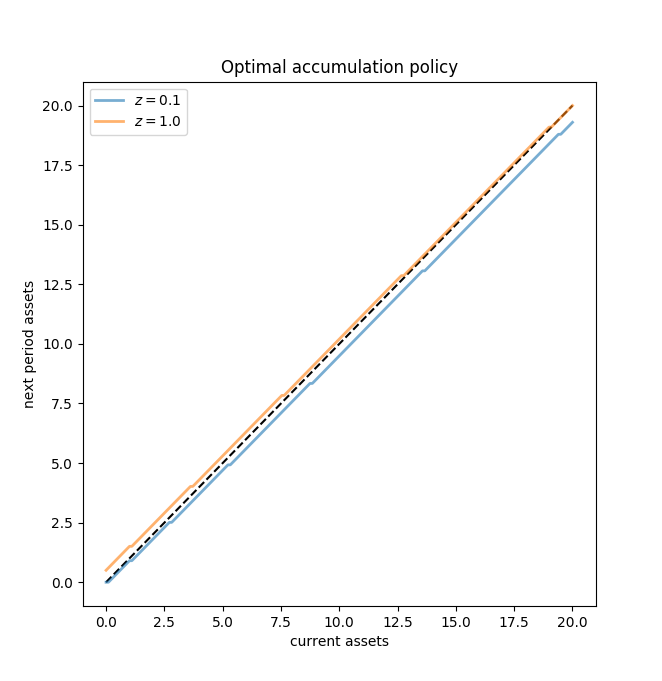
\includegraphics[scale = 0.8]{accumulation_policy.png}
\end{figure}

After that, the equilibrium is calculated visually: last part of the code draws aggregate supply and demand curves. The intersection gives equilibrium interest rates and capital, as can be seen in figure \ref{plot:equilibrium}.
\begin{figure}[]
\centering
\caption{Example of equilibrium for Aiyagari model.}
\label{plot:equilibrium}
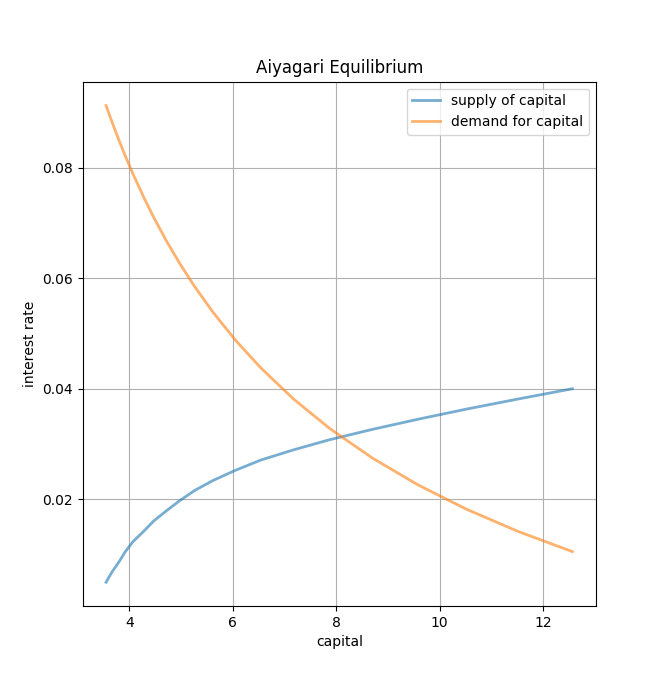
\includegraphics[scale = 0.8]{equilibrium.png}
\end{figure}
.

\newpage
\section{Conclusion}
This paper only deals with a restriction of Aiyagari's original works. Such economist's later research ranges from setting taxes to marriage patterns and it would be interesting to explore numerical solutions to these settings. \\
As for Aiyagari-Bewley model, a recent extension can be found in \cite{aiyacont}. The model is here presented in a continuous-time version and modern software tools allow to solve such extension numerically.

\newpage
\listoffigures

\begin{thebibliography}{99}
\bibitem[Bewley (1986)]{bewley} {\sc Bewley, T.} (1986).  \textit{Stationary Monetary Equilibrium With a Continuum of Independently Fluctuating Consumers}. Contributions to Mathematical Economics in Honor of Gérard Debreu.

\bibitem[Aiyagari (1994)]{aiya94} {\sc Aiyagari, S. R.} (1994). \textit{UNINSURED IDIOSYNCRATIC RISK AND AGGREGATE SAVING}. The Quarterly Journal of Economics, 109, Oxford University Press.
\bibitem[Aiyagari (1993)]{aiya93} {\sc Aiyagari, S. R.} (1993). \textit{Uninsured Idiosyncratic Risk and Aggregate Saving}. Research Department Working Paper 502, Federal Reserve Bank of Minneapolis.
\bibitem[QuantEcon (1)]{quantecdisc} {\sc QuantEcon.}  \textit{The Aiyagari Model.} \texttt{https://python.quantecon.org/aiyagari.html}

\bibitem[Achdou et al. (2017)]{aiyacont} {\sc Achdou, Y.}, {\sc Han, J.}, {\sc Lasry J. M.}, {\sc Lions P. L.} amd {\sc Moll, B.} (2017). \textit{Income and Wealth Distribution in Macroeconomics: A Continuous-Time Approach}. Princeton University.
\end{thebibliography}
\end{document}